% Results: Studies 1 to 5, then the exploratory cross-study analyses; every number through a macro in generated/numbers.tex.
% Statuses and verdicts follow notes/argument.md and notes/results_ledger.md. American spelling.
% The detail behind this section is in the Supplementary Notes (supplement/sections/note*.tex),
% numbered in the order this section first cites them.

Fig.~\ref{fig:design} and Table~\ref{tab:summary} summarize the five studies. By credit we mean the ratings people gave a work, not judgments of authorship. The \NTotal{} analyzed records are participations, not people: they came from \NPeople{} students in the UCLA Psychology subject pool, \NPeopleRepeat{} of whom took part in two studies, all for course credit.

Supplementary Table~1 lists every registered test with its status and verdict. A $p$-value is the chance of a difference at least this large if there were no effect, and a result is significant when $p$ is below .05. A 95\% confidence interval (CI) is the range of values the data do not rule out at the 95\% level. A registered confirmatory test is decided by its registration's rule, usually after Holm's correction,\cite{holm1979simple} which raises each $p$-value in a set of tests so that the chance of calling any result in the set significant by mistake stays at .05. A registered secondary test lies outside that set and is uncorrected unless stated. A registered description is an estimate that a registration asks us to report without a test of its own, and a descriptive result carries no test. An exploratory analysis was named as exploratory in a registration or not named at all; the analyses that pool Studies 2, 4 and 5, the image check and the breakdown of Study~5's interaction were specified on 9 and 10 October 2026, after the registered results were known. Because every registration followed data collection, and for Studies 1 to 4 followed analyses of the same data (Table~\ref{tab:summary}), `registered' means written into a registration, not fixed before collection.

\begin{figure}[tbp]
\centering
\makebox[\textwidth][c]{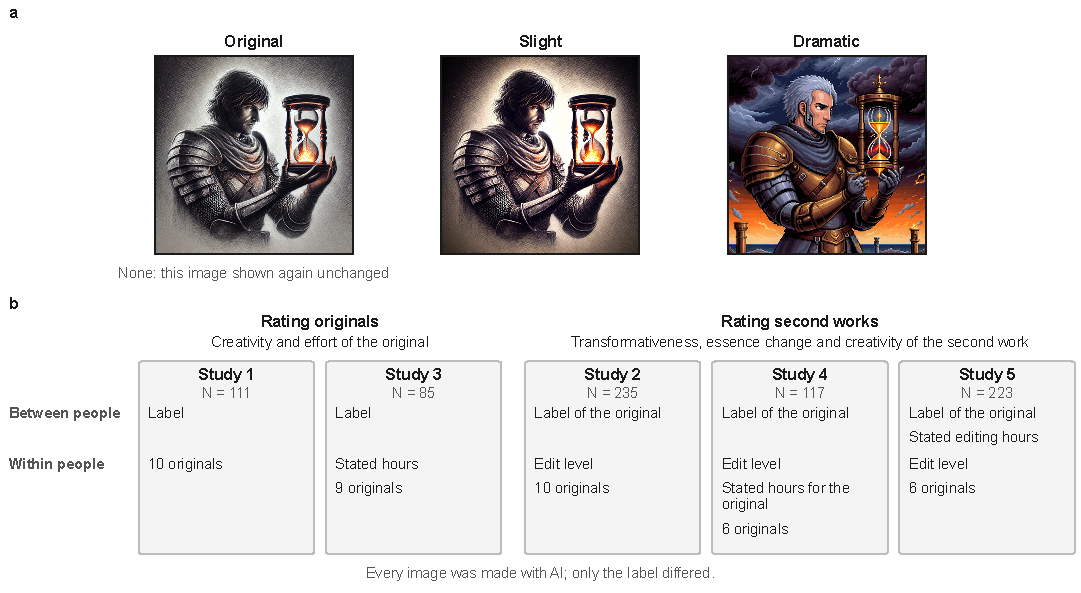
\includegraphics[width=183mm]{fig1_design}}
\caption{\textbf{Design of the five studies.} \textbf{a},~One of the ten originals and its Slight and Dramatic versions, which we edited by hand. In Studies 2, 4 and 5 the original was also shown again unchanged, as the None second work, so each second work's edit level was None, Slight or Dramatic, and each second work appeared beside its original. Of the ten Slight versions, \XSImageCheckSlightReframedN{} were also cropped or resized; the one shown was not. \textbf{b},~What each study varied between participants (each person saw one condition) and within participants (each person saw every condition), what participants rated and how many were analyzed ($N$). The label said that the artist, Alex, made the original with design and sketching tools (Human label) or by prompting an AI system (AI label). Every original was made with OpenAI's DALL\textperiodcentered E, used through ChatGPT, so the Human label was a cover story, and each participant saw one label throughout. In Studies 2, 4 and 5, both label groups read that Alex made the second works with his design and sketching tools, so the label described only the original. Stated times were under 1 hour, 10 hours or 100 hours; Study~3's were hours of drawing under the Human label and of revising prompts under the AI label. Study~5 also stated a time for the original, but a fault in the survey script left its record blank, so it is not analyzed. The studies ran in the order 2, 4, 1, 3, 5, and all five were registered after data collection: their hypotheses and analyses were filed on the Open Science Framework, an online archive for study plans, which has nothing to do with copyright registration.}
\label{fig:design}
\end{figure}

% Table 1: the five studies at a glance. One row per study: what it asked, the answer its
% registered tests gave, and when it was run relative to its registration. Written by
% tools/make_tables.py; do not edit by hand. Numbers come only from generated/numbers.tex;
% verdicts follow notes/results_ledger.md and are checked against the pipeline tables.
% Needs booktabs and caption, both loaded in main.tex.
\begin{table}[tbp]
\centering
\caption{\textbf{The five studies at a glance.} Supplementary Table~1 lists every registered test and its verdict; Supplementary Table~2 gives the label's effect on second works, with intervals.}
\label{tab:summary}
\normalsize
\setlength{\tabcolsep}{5pt}
\begin{tabular}{@{}p{40pt}p{128pt}p{\dimexpr\textwidth-250pt-6\tabcolsep\relax}p{82pt}@{}}
\toprule
Study & What it asked & Registered answer & Order run; registered\tabularnewline
\midrule
\multicolumn{4}{@{}p{\textwidth}@{}}{\raggedright\textbf{Originals: the same AI-made images, rated for creativity and effort}}\\*
\addlinespace[2pt]
\raggedright Study~1\newline $N$~=~\SOneN & \raggedright Does the AI label lower both ratings (H1), effort more (H2), alike with or without a human figure (H3), and spread them more between people (H4)? & \raggedright H1 and H2: supported. H3: supported on effort, inconclusive on creativity. H4: not supported as registered. & \raggedright Ran third; registered after its analyses\tabularnewline
\addlinespace[3pt]
\raggedright Study~3\newline $N$~=~\SThreeN & \raggedright With under 1, 10 or 100 hours stated, does the gap (the penalty) close by 100 hours? & \raggedright Decision on both ratings: the gap persists. The AI label lowered ratings and stated time raised them (both supported); a change in the gap with time was not significant. & \raggedright Ran fourth; registered after an Apr. 2025 analysis and a Sept. 2025 talk\tabularnewline
\addlinespace[3pt]
\midrule
\multicolumn{4}{@{}p{\textwidth}@{}}{\raggedright\textbf{Second works: Alex's edits of each labeled original, at three levels}}\\*
\addlinespace[2pt]
\raggedright Study~2\newline $N$~=~\STwoN & \raggedright Do ratings of a second work rise with the level of edit (H1)? Is the label's effect small (H2), and does it shrink from None to Dramatic (H3)? & \raggedright H1 holds on every measure. H2, over the three measures: not shown to be small (small or absent on transformativeness and essence change; not shown to be small on creativity). H3: not significant. & \raggedright Ran first; registered after a Feb. 2025 analysis\cite{kamper2025originalsin} and a Sept. 2025 talk\tabularnewline
\addlinespace[3pt]
\raggedright Study~4\newline $N$~=~\SFourN & \raggedright Study~2's H1 and H2 again, and do hours stated for the original change ratings of the second work (H3)? & \raggedright H1 supported. H2, over the three measures: not shown inside the bound (inside it on essence change only, a pass lost in the registered refit\textsuperscript{a}). H3: not significant. & \raggedright Ran second; registered after a Feb. 2025 analysis\cite{kamper2025originalsin} and a Sept. 2025 talk\tabularnewline
\addlinespace[3pt]
\raggedright Study~5\newline $N$~=~\SFiveN & \raggedright Do hours stated for the edit change ratings of the second work, or the label's effect on them? & \raggedright Editing hours: absent or small, inside $\pm$\SFiveEditTimeBound. A change in the label's effect with editing hours: significant on creativity only. The label's effect (secondary): significant, not inside the bound, at Slight on every measure and at Dramatic on transformativeness. & \raggedright Ran last; registered before any rating was averaged or compared by label\tabularnewline
\bottomrule
\end{tabular}
\par\smallskip
{\small\raggedright Every original was AI-made (OpenAI's DALL\textperiodcentered{}E, used through ChatGPT). Human label: Alex used design and sketching tools; AI label: he prompted an AI system. \emph{Penalty}: Human-label minus AI-label mean rating on 1-to-5 scales (the gap, in Study~3's registration). \emph{None, Slight, Dramatic}: the original shown again unchanged, a light edit, a heavy edit; the measures: transformativeness, essence change, creativity. \emph{Supported}, \emph{holds}: passed by the registration's rule. \emph{Significant}: $p$ below .05, after Holm's correction for confirmatory tests (which holds the chance of any false positive in a study's confirmatory set at .05) and uncorrected for \emph{secondary} tests outside that set. \emph{Small or absent}, \emph{inside the bound}: an equivalence test placed the effect inside $\pm$\SourceBound{} points, half of Study~1's creativity penalty ($\pm$\SFiveEditTimeBound, Study~3's creativity time effect, for editing hours); small, not zero. \emph{Not shown to be small}, \emph{not shown inside}: that test failed, which does not show an effect. \emph{Inconclusive}: no effect and a small one could not be told apart. \textsuperscript{a}Without the \SFourMachineMadeN{} Human-label participants who wrote that a machine made the work. All five registrations were filed on 8 October 2026, after data collection.\par}
\end{table}


\subsection*{An AI label lowers credit for the same image, more for effort than creativity}

Study~1's \SOneN{} participants rated all ten originals on 1-to-5 scales for creativity (`How much creativity was involved in the production of this work? Creativity is defined as the presence of at least a minimal original, intellectual contribution to the creation of the work.') and for effort (`How much effort was involved in the production of this work?', with no definition). Each estimate is a difference between predicted mean ratings from a linear mixed model, a regression that gives each participant and each image its own baseline. We call the Human-label minus AI-label difference the label's penalty; a positive penalty means that the AI label lowered the rating. With no unlabeled condition, `lowered' means lower than under the Human label.

The AI label lowered both ratings of the same images: by \SOneHOneCreatDiff{} points on creativity (95\% CI \SOneHOneCreatLo{} to \SOneHOneCreatHi; Holm $p$~\SOneHOneCreatPHolm; Fig.~\ref{fig:penalty}a) and by \SOneHOneEffDiff{} points on effort (\SOneHOneEffLo{} to \SOneHOneEffHi; Holm $p$~\SOneHOneEffPHolm). The effort penalty was larger by \SOneHTwoDiff{} points (\SOneHTwoLo{} to \SOneHTwoHi; Holm $p$~\SOneHTwoPHolm; Fig.~\ref{fig:penalty}a, gray row), and an ordinal model, which treats the five answers as ordered categories rather than evenly spaced numbers, agreed ($p$~\SOneHTwoOrdP). Under the Human label, effort sat above creativity (\SOneMeanHumanEff{} against \SOneMeanHumanCreat); under the AI label, it sat below (\SOneMeanAIEff{} against \SOneMeanAICreat). These results pass Study~1's registered confirmatory tests of H1, that the AI label lowers both ratings, and H2, that it lowers effort more. But both drops had been seen in $t$-tests (comparisons of two means) in April 2025, and the larger drop on effort in a talk in September 2025, before the model and correction were chosen, so H1 and H2 are registered tests of patterns already seen, not predictions. Only the creativity item carried a definition, so part of the H2 difference may come from the wording of the items. Study~1's H3, that the penalty is the same for images with and without a human figure, was decided outside the confirmatory set by its own registered rule, against a bound set after the analyses. It was supported on effort and inconclusive on creativity, where the design could not tell no difference from a small one. H4, a registered confirmatory test that the AI label spreads ratings more between people and less within each person, met its criterion on effort only, so it was not supported as registered (Supplementary Note~1 and Supplementary Fig.~1).

A registered robustness check (descriptive) refit the penalty \SOneSpecN{} ways for each rating, and in all \SOneSpecNTotal{} versions the AI label still lowered the rating. Of the \SOneBeliefNHuman{} Human-label participants, \SOneBeliefNarrowN{} wrote at least once that a work is or looks machine-made, by a word list written after results by label had been read; this is a count of statements, not of disbelief. Disbelief in the cover story would shrink the penalty, not create it, and a registered refit without those participants enlarged it, to \SOneBeliefRefitCreatDiff{} points on creativity and \SOneBeliefRefitEffDiff{} on effort. Dropping low raters can enlarge a penalty by arithmetic alone. Random Human-label groups of the same size and mean effort rating enlarged the creativity penalty, measured against the spread of ratings, as much as the exclusion did, but never enlarged the effort penalty that far; so on effort the enlargement is not explained by that arithmetic, and these data say nothing more about its cause (exploratory description; Supplementary Note~2).

\subsection*{Stated hours raised ratings but did not close the gap within 100 hours}

Study~3 tested a rival account named in its registration, which we call the effort-signal account. On it, the AI label lowers ratings only because it signals little work, so stating that Alex spent 100 hours on an image should shrink the penalty (the registration's gap) to almost nothing. Study~3's \SThreeN{} new participants each rated nine originals, three at each stated time: under 1 hour, 10 hours or 100 hours. Under the Human label Alex spent those hours drawing; under the AI label he spent them revising prompts, so there more time also meant more control over the image, and the two cannot be told apart. The registered rule called the gap persistent if its 95\% CI at 100 hours lay above zero and it failed an equivalence test, which asks whether an effect is shown to lie inside a stated bound, here $\pm$\SourceBound{} points (half of Study~1's creativity penalty).\cite{schuirmann1987comparison,lakens2017equivalence}

On both ratings, the registered decision was that the gap persists. At 100 hours, the gap's 90\% CI, the interval that matches an equivalence test, ran from \SThreeCreatGapHundredLoNinety{} to \SThreeCreatGapHundredHiNinety{} points on creativity and from \SThreeEffGapHundredLoNinety{} to \SThreeEffGapHundredHiNinety{} on effort, and both 95\% CIs lay above zero. This does not refute the effort-signal account: both 90\% CIs reach below \SourceBound, so part of the gap may still come from how little work the AI label implies, especially on effort.

The registered confirmatory $F$ tests for label and for time, which ask whether a factor changes the mean rating, survived Holm's correction on both ratings; by the estimates, the AI label lowered both ratings and stated time raised both. Averaged over labels, 100 hours minus under 1 hour was \SThreeCreatTimeContrastEst{} points on creativity (95\% CI \SThreeCreatTimeContrastLo{} to \SThreeCreatTimeContrastHi), most of it between 10 and 100 hours, and \SThreeEffTimeContrastEst{} on effort (\SThreeEffTimeContrastLo{} to \SThreeEffTimeContrastHi). A change in the gap with time (the label-by-time interaction) did not survive Holm's correction on either rating, and no test of equal rises under the two labels was registered. As registered description, the creativity gap was \SThreeCreatGapUnderOneHourEst, \SThreeCreatGapTenHoursEst{} and \SThreeCreatGapHundredHoursEst{} points at under 1, 10 and 100 hours, and the effort gap was \SThreeEffGapUnderOneHourEst, \SThreeEffGapTenHoursEst{} and \SThreeEffGapHundredHoursEst{} (Fig.~\ref{fig:penalty}a). Each effort gap was smaller than Study~1's effort penalty of \SOneHOneEffDiff, an untested comparison across studies. With time stated, the two gaps were close (at 10 hours the effort gap was the smaller), and Study~3 registered no test of effort against creativity, so the larger drop on effort rests on Study~1 (Supplementary Note~3).

\begin{figure}[tbp]
\centering
\makebox[\textwidth][c]{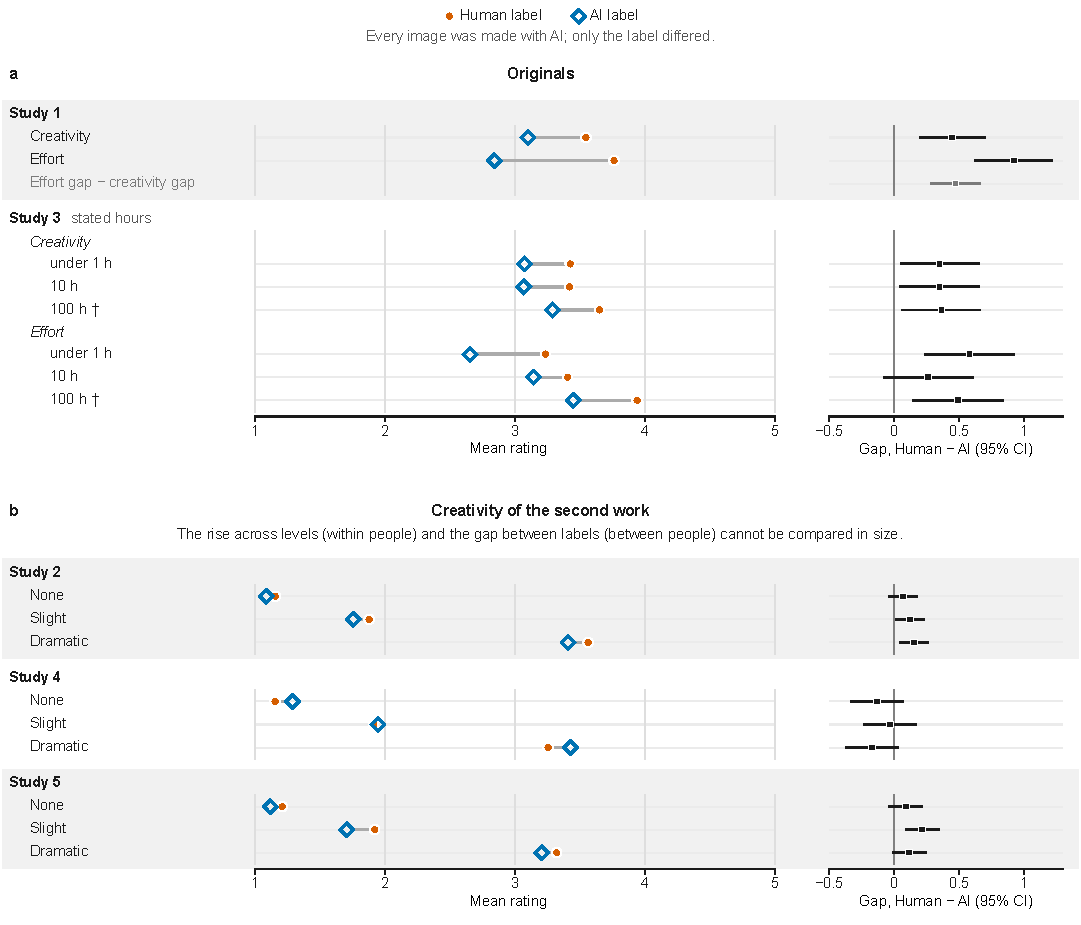
\includegraphics[width=183mm]{fig2_results}}
\caption{\textbf{Mean ratings under the two labels, and the gap between them.} Circles and diamonds are the two label groups' mean ratings (1 to 5), as predicted by each study's statistical model (Methods). Squares are the gap, the Human-label mean minus the AI-label mean (called the penalty in the text), at the same scale as the ratings, with its 95\% confidence interval (CI). Right of zero, the AI label lowered the rating. Judge a gap by its CI, not by whether the marks overlap; a CI that crosses zero does not show a gap of zero. `Registered' means written into a registration filed after data collection, not copyright registration. \textbf{a},~Originals. Study~1's gaps are registered confirmatory tests of H1, that the AI label lowers both ratings, and its gray row tests H2, that it lowers effort more; all three passed after Holm's correction. Study~3's gaps are registered description, estimates its registration names with no test of their own. The 100-hour gaps (\dag) entered the registered decision, which was that the gap persists. \textbf{b},~Creativity of the second work, asked as the creativity involved in its production; None is the original shown again unchanged. Each person saw every level but only one label. The gaps are exploratory in Study~2 and registered secondary tests in Studies 4 and 5, outside each study's confirmatory set (Supplementary Table~1) and judged at .05 without correction. They average over the hours stated for the original (Study~4) or over stated editing hours (Study~5, whose creativity gap differed across them; Supplementary Fig.~2). Supplementary Fig.~3 shows the other two ratings; Supplementary Table~2 lists the registered tests. No test compared rows from different studies.}
\label{fig:penalty}
\end{figure}

\subsection*{Ratings of Alex's second work follow the level of modification}

Studies 2, 4 and 5 changed two things. The rated act became Alex's edit, described in the same words to both label groups, and his part became visible as a before-and-after pair. Each original appeared beside three second works: None, the original shown again unchanged; Slight, a light edit; and Dramatic, a heavy one. Participants rated each second work's transformativeness, how much it adds new expression, meaning or message to the original (a lay rating whose wording echoes court decisions on fair use, the rule that allows some copying without permission; it is not a fair-use judgment). They also rated its essence change, how much the original's essence changed (defined in Studies 4 and 5 as its core sense and feeling), and the creativity involved in its production. The label now described an act the questions did not ask about, so any effect it had is a carry-over from what was said about the original. Three accounts predict different carry-overs. Under taint, the AI origin passes to anything built from it, so the penalty is the same at every level and, at full strength, as large as on originals. Under dilution, it is largest at None and shrinks as the edit grows. Under severance, the label does not reach second works at all. These studies also differed from Studies 1 and 3 in participants, timing, label wording, how many originals each person saw (six of the ten in Studies 4 and 5) and measures (effort was not rated, and Study~2's creativity item carried no definition), so every comparison between originals and second works is a reading across studies, not a test.

Ratings rose steeply with the level of modification (H1 in Studies 2 and 4, registered confirmatory; creativity in Fig.~\ref{fig:penalty}b). In both studies every step was positive and significant after Holm's correction on all three measures (every Holm $p$~\STwoCreatSlightMinusNonePHolm), by \STwoCreatSlightMinusNoneEst{} to \SFourTransSlightMinusNoneEst{} points from None to Slight and \SFourCreatDramaticMinusSlightEst{} to \STwoTransDramaticMinusSlightEst{} from Slight to Dramatic. The ordinal model agreed, except on Study~2's creativity ratings, where its fit did not converge (its fitting procedure settled on no solution), so that check is not completed. Study~5's predicted means rose the same way (descriptive). In an exploratory check in which two image-recognition networks measured each edited image's distance from its original,\cite{oquab2024dinov2,radford2021learning} every Slight version lay closer to its original than the Dramatic version did, but within a level, ratings are not shown to track the amount of visible change (descriptive; Supplementary Note~4). At None, means in Studies 2 and 4 sat near the floor of the scale (\STwoTransMeanNone{} to \SFourCreatMeanNone), leaving little room for a label effect. Because the label varied between participants and the level within them, the sizes of their effects cannot be compared.

\subsection*{The AI label's effect on the second work is much less than on originals, but not nothing}

Studies 2, 4 and 5 asked whether the label's penalty on a second work lay inside a registered bound of $\pm$\SourceBound{} points, half of Study~1's creativity penalty on originals (\SOneHOneCreatDiffPrecise{} points before rounding; Fig.~\ref{fig:penalty}b; Supplementary Table~2). Judged alone, an equivalence test passes when the penalty's 90\% CI lies wholly inside the bound; inside a Holm-corrected set, it can fail even then. A pass means that the penalty is small, not zero; a failure means only that it is not shown to be small.

Averaged over levels, the penalty was shown inside the bound in \NHTwoPassSTwoSFour{} of the \NHTwoTestsSTwoSFour{} registered confirmatory tests (Study~2's and Study~4's H2): transformativeness and essence change in Study~2, and essence change in Study~4. H2 asked for a small effect on every measure, so as registered it holds in neither study. Study~2's creativity penalty, \STwoCreatPenaltyEst{} (90\% CI \STwoCreatPenaltyLoNinety{} to \STwoCreatPenaltyHiNinety), was not shown to be small: its uncorrected interval lay inside the bound, but the test failed after Holm's correction (Holm $p$~\STwoCreatPenaltyPHolm). That penalty had already appeared in our published analysis of these data,\cite{kamper2025originalsin} run by February 2025, in which this study is Study~1, so this test re-analyzes an effect already known. Study~4's transformativeness test also failed only after correction (Holm $p$~\SFourTransPenaltyPHolm), and its creativity estimate ran the other way (\SFourCreatPenaltyEst; 90\% CI \SFourCreatPenaltyLoNinety{} to \SFourCreatPenaltyHiNinety), not significantly. In a registered refit without the \SFourMachineMadeN{} Human-label participants who wrote that a machine made the work, Study~4's essence-change pass was lost (Holm $p$~\SFourEssPenaltyPHolm{} on the full sample, Holm $p$~\SFourEssPenaltyPHolmRefitPrecise{} in the refit), the only one of the refit's \SFourNRefitVerdicts{} verdicts to change.

Study~5 registered the penalty at each level as secondary tests, judged without correction. At None, where ratings sit near the floor, the penalty lay inside the bound on all three measures. At Slight, it was significant and not shown inside the bound on all three: \SFiveTransPenaltySlightEst{} points on transformativeness ($p$~\SFiveTransPenaltySlightP), \SFiveEssPenaltySlightEst{} on essence change ($p$~\SFiveEssPenaltySlightP) and \SFiveCreatPenaltySlightEst{} on creativity ($p$~\SFiveCreatPenaltySlightP). Each of these estimates is under \SourceBound, so `not inside the bound' means not shown to be small, not shown to be large. They also average over the three stated editing times, and in an exploratory breakdown the Slight creativity penalty rests largely on the 10-hour groups (next section; Supplementary Note~5 and Supplementary Fig.~2). At Dramatic, transformativeness was also significant and not inside the bound (\SFiveTransPenaltyDramaticEst), essence change lay inside it, and creativity was inconclusive (\SFiveCreatPenaltyDramaticEst; its 90\% CI reached \SFiveCreatPenaltyDramaticHiNinetyPrecise, just past the bound). Study~4 registered the same tests at each level as secondary tests. At Slight they, too, found penalties that were significant and not shown inside the bound on transformativeness and essence change, while the creativity penalty lay inside the bound (Fig.~\ref{fig:penalty}b and Supplementary Fig.~3; Supplementary Note~6).

Across the \NSourceEquivTests{} registered equivalence tests on second works, every point estimate was smaller than \SourceBound{} in size, but only \NSourceEquivPass{} tests showed the penalty inside the bound. Read across studies rather than tested, every registered interval for the creativity penalty on second works excludes Study~1's full penalty of \SOneHOneCreatDiffPrecise{} points, the size that full-strength taint predicts, although several overlap that penalty's own 95\% CI (\SOneHOneCreatLo{} to \SOneHOneCreatHi). On this reading, the label carried much less into creativity ratings of second works than into creativity ratings of originals; creativity is the only measure rated on both. What it did carry, which we call the residue, was small on average, uneven across studies and detectable at slight edits in Study~5 on every measure and in Study~4 on transformativeness and essence change; in Study~5 the exploratory breakdown places most of it in the 10-hour groups.

\subsection*{No detectable carry-over from hours stated for the original, and no detectable effect of stated editing hours on average}

Study~4 stated how long Alex had spent on each original, and each participant saw every stated time. The hours did not significantly change ratings of the second work on any measure, alone or by level of modification (Study~4's H3, confirmatory; every Holm $p$~\SFourCreatSourceTimePHolm), and the ordinal model agreed. As registered secondary tests, 100 hours minus under 1 hour lay inside $\pm$\SourceBound{} points on all three measures (transformativeness \SFourTransTimeContrastEst, essence change \SFourEssTimeContrastEst, creativity \SFourCreatTimeContrastEst), and no change in the label's penalty across those hours was detected (not significant). Our published analysis of these data,\cite{kamper2025originalsin} in which this study is Study~2, reported an effect of these hours on creativity that the registered model does not reproduce.

Study~5 stated how long Alex had spent making the second work, one time per participant for the whole session. Averaged over the two labels, stated editing hours did not detectably change ratings (confirmatory; every Holm $p$~\SFiveCreatEditTimePHolm). Against a bound of $\pm$\SFiveEditTimeBound{} points, the size of Study~3's creativity time effect, the registered secondary equivalence tests (uncorrected) read `absent or small: inside the bound' on all three measures. On creativity, 100 hours minus under 1 hour was \SFiveCreatEditTimeContrastEst{} points (90\% CI \SFiveCreatEditTimeContrastLoNinety{} to \SFiveCreatEditTimeContrastHiNinety), so effects up to about \SFiveCreatEditTimeContrastHiNinety{} remain compatible. Neither Study~4 nor Study~5 rated effort, on which Study~3's time effect was largest.

Only \SFiveNConfirmatoryHolmSignificant{} of Study~5's \SFiveNConfirmatory{} registered confirmatory tests passed: the label's creativity penalty differed across stated editing times ($F$(\SFiveCreatSourceByEditTimeDfNum,~\SFiveCreatSourceByEditTimeDfDen)~=~\SFiveCreatSourceByEditTimeF, Holm $p$~\SFiveCreatSourceByEditTimePHolm), and the registered ordinal check and a reanalysis with every item rescaled from 0 to 1 agreed. Rather than shrinking as the hours rose, as the registration had sketched, the penalty in an exploratory, uncorrected breakdown (Supplementary Note~5 and Supplementary Fig.~2) was small at under 1 hour and largest at 10 hours, where it reached \XSTimeCheckSFiveCreatPenaltyTenHoursSlightEst{} at Slight and \XSTimeCheckSFiveCreatPenaltyTenHoursDramaticEst{} at Dramatic, about as large as on originals, read across studies. At 100 hours it reversed at Dramatic (\XSTimeCheckSFiveCreatPenaltyHundredHoursDramaticEst). Each label-by-time combination was a separate group of \SFiveNCellMin{} to \SFiveNCellMax{} people, and the 10-hour groups also showed the largest penalties on the other two measures, whose registered interactions were not significant. A single 10-hour group that happened to rate unusually could produce this pattern on all three measures and inflate Study~5's Slight and Dramatic estimates; with the corrected $p$ just under .05, the interaction may also be a chance result that survived correction.

\subsection*{In an exploratory pooling of Studies 2, 4 and 5, the residue was largest at slight edits}

Specified after every registered result was known, this analysis is uncorrected and changes no registered verdict (Supplementary Note~6; Supplementary Fig.~4). A model that fitted Studies 2, 4 and 5 together, each weighted equally, put the creativity penalty at \XSCreatPenaltyNoneEst, \XSCreatPenaltySlightEst{} and \XSCreatPenaltyDramaticEst{} points at None, Slight and Dramatic; its fits were singular, meaning one of the sources of variation the model allows for was estimated at zero. On all three measures the Slight penalty lay above the average of the None and Dramatic penalties, and no fall from None to Dramatic was shown, so the pattern dilution predicts did not appear, though the floor at None weakens that test. The pooled curve averages over studies that disagree on creativity: without Study~4, whose estimates lay below zero (none significantly), the Slight penalty rose to \XSCreatPenaltyWithoutSFourSlightEst{} and its 90\% CI (\XSCreatPenaltyWithoutSFourSlightLoNinety{} to \XSCreatPenaltyWithoutSFourSlightHiNinety) extended past the bound. Two standard scores for choosing between models disagreed: AIC (Akaike's information criterion) favored a penalty that differs by level, and BIC (the Bayesian information criterion), which charges more for each added quantity a model estimates, favored no penalty at all, as severance predicts. The residue was not confined to Slight: Study~2's creativity penalty (exploratory) and Study~5's transformativeness penalty (registered secondary) were significant at Dramatic.

\subsection*{What the explanations referred to}

This section is exploratory (Supplementary Note~7). Eight fixed word lists, applied by a script blind to label and rating, flagged what each written explanation mentioned. Because each explanation followed its rating, these results describe what the words referred to, not why anyone rated as they did. On originals, what `effort' referred to depended on the label. In Study~1, \SOneTextEffortDetailPct{} of Human-label effort explanations named visible detail, and \SOneTextPromptEffortAIPct{} of AI-label effort explanations mentioned prompting or machines, against \SOneTextPromptEffortHumanPct{} under the Human label; Study~3 showed the same shift (uncorrected). On second works, the label left only a faint trace. AI-label explanations mentioned prompting or a machine more often than Human-label ones, but rarely (at most \XSOriginTalkAIDramaticPct), and no difference was shown in how far a person's explanations changed from None to Dramatic, where taint predicts less change under the AI label. No study asked participants to recall the label (a manipulation check).
